%==============================================================================
% Sjabloon onderzoeksvoorstel bachelorproef
%==============================================================================
% Gebaseerd op LaTeX-sjabloon ‘Stylish Article’ (zie voorstel.cls)
% Auteur: Jens Buysse, Bert Van Vreckem
%
% Compileren in TeXstudio:
%
% - Zorg dat Biber de bibliografie compileert (en niet Biblatex)
%   Options > Configure > Build > Default Bibliography Tool: "txs:///biber"
% - F5 om te compileren en het resultaat te bekijken.
% - Als de bibliografie niet zichtbaar is, probeer dan F5 - F8 - F5
%   Met F8 compileer je de bibliografie apart.
%
% Als je JabRef gebruikt voor het bijhouden van de bibliografie, zorg dan
% dat je in ``biblatex''-modus opslaat: File > Switch to BibLaTeX mode.

\documentclass{voorstel}

\usepackage{lipsum}

%------------------------------------------------------------------------------
% Metadata over het voorstel
%------------------------------------------------------------------------------

%---------- Titel & auteur ----------------------------------------------------

% TODO: geef werktitel van je eigen voorstel op
\PaperTitle{Vergelijking Tussen Keuzes en Combinaties van TypeScript Transpilers en JavaScript Bundlers Bij het Ontwikkelen van React Applicaties}
\PaperType{Onderzoeksvoorstel Bachelorproef 2021-2022} % Type document

% TODO: vul je eigen naam in als auteur, geef ook je emailadres mee!
\Authors{Nicolas Van Damme\textsuperscript{1}} % Authors
\CoPromotor{Arvid De Meyer\textsuperscript{2} (Codifly)}
\affiliation{\textbf{Contact:}
  \textsuperscript{1} \href{mailto:nicolas.vandamme@student.hogent.be}{nicolas.vandamme@student.hogent.be};
  \textsuperscript{2} \href{mailto:arvid.de.meyer@codifly.be}{arvid.de.meyer@codifly.be};
}

%---------- Abstract ----------------------------------------------------------

\Abstract{
    Een paar jaar geleden was de keuze van transpiler en bundler voor een React project niet zo moeilijk. De keuzes waren beperkt en concurrentie bestond amper. In de loop van de laatste paar jaar is daar echter veel beweging in gekomen. Nieuwe opties worden steeds aantrekkelijker, maar is het 2022 echter al een goed idee om een overstap te maken? De onderzoeker tracht te achterhalen welke opties een goede match vormen met Codifly, een bedrijf dat zich specialiseert in het ontwikkelen van React en React Native applicaties.
}

%---------- Onderzoeksdomein en sleutelwoorden --------------------------------
% TODO: Sleutelwoorden:
%
% Het eerste sleutelwoord beschrijft het onderzoeksdomein. Je kan kiezen uit
% deze lijst:
%
% - Mobiele applicatieontwikkeling
% - Webapplicatieontwikkeling
% - Applicatieontwikkeling (andere)
% - Systeembeheer
% - Netwerkbeheer
% - Mainframe
% - E-business
% - Databanken en big data
% - Machineleertechnieken en kunstmatige intelligentie
% - Andere (specifieer)
%
% De andere sleutelwoorden zijn vrij te kiezen

\Keywords{Mobiele applicatieontwikkeling. TypeScript --- Transpilatie --- Bundling} % Keywords
\newcommand{\keywordname}{Sleutelwoorden} % Defines the keywords heading name

%---------- Titel, inhoud -----------------------------------------------------

\begin{document}

\flushbottom % Makes all text pages the same height
\maketitle % Print the title and abstract box
\tableofcontents % Print the contents section
\thispagestyle{empty} % Removes page numbering from the first page

%------------------------------------------------------------------------------
% Hoofdtekst
%------------------------------------------------------------------------------

% De hoofdtekst van het voorstel zit in een apart bestand, zodat het makkelijk
% kan opgenomen worden in de bijlagen van de bachelorproef zelf.
\setlength{\parskip}{0.2em}
%---------- Inleiding ---------------------------------------------------------

\section{Introductie} % The \section*{} command stops section numbering
\label{sec:introductie}
Dynamische webapplicaties zijn onmogelijk zonder een ondersteunende programmeertaal. Binnen Codifly en zeer veel andere bedrijven komt die in de vorm van JavaScript. Doorheen de jaren zijn veel hulpmiddelen gekomen en gegaan om de ontwikkelaars van zulke webapplicaties te ondersteunen. Van het omzetten van de ene taal naar de andere, tot automatische samenbundeling van je code. In deze paper zal gekeken worden naar verschillende TypeScript transpilers en JavaScript bundlers, om zo hopelijk te kunnen concluderen welke TypeScript transpilers en JavaScript bundlers het waard zijn om een oog op te houden, welke voor- en nadelen ze hebben, en of bepaalde combinaties een synergie hebben met elkaar bij ontwikkeling van React applicaties in het algemeen. Verder zal na het achterhalen van welke transpilers en bundlers Codifly momenteel in gebruik neemt er aan de hand van een proof-of-concept dan ook geanalyseerd kunnen worden welke mogelijke positieve invloed een andere keuze zou kunnen hebben binnen het ontwikkelingsproces van Codifly.

%---------- Stand van zaken ---------------------------------------------------

\section{State-of-the-art}
\label{sec:state-of-the-art}

\subsection{De limitaties van JavaScript}
Binnen het gebied van webontwikkeling wordt zeer vaak met JavaScript in contact gekomen. JavaScript heeft echter bepaalde limitaties die het ontwikkelingsproces kunnen hinderen. \autocite{geeksforgeeks_2021}

Alle programmeertalen zijn tot op een zekere mate zwak/sterk getypeerd, en dynamisch/statisch getypeerd. In een dynamisch getypte taal hebben alle waarden een type aan zich verbonden tijdens runtime\footnote{Wanneer de applicatie uitgevoerd wordt.}. JavaScript, een dynamisch getypte taal, houdt paren van een waarde en type bij; bijvoorbeeld (Number, 4). Een statisch getypte taal moet dit niet doen, aangezien we variabelen expliciet een type geven in onze broncode.

De mate waarin een taal sterk of zwak getypeerd is hangt af van hoe strikt de taal types afdwingt. De \lq type coercion \rq die een taal aanbiedt is hier een typisch voorbeeld van. Type coercion is het proces van het omzetten van waarden van het ene type naar het andere. Als men in JavaScript een variabele declareren als volgt:

\verb|const waarde = true + false|

Dan zal waarde het nummer 1 bevatten. JavaScript zet eerst de booleaanse waarden om naar nummers om ze op te tellen. Wat je gedaan hebt is dus effectief:

\verb|const waarde = 1 + 0|

In een sterk getypte taal zal dit veel strenger afgedwongen worden, maar de exacte limitaties hangen nog steeds van taal tot taal af. Welke soort typering het beste is, is geen eenzijdige discussie. Onderzoek van \textcite{meijer_drayton_2004} ondersteund de notie dat het gebruik van dynamische typering in een statisch getypte omgeving een gulden middenweg is.

\subsection{Exit JavaScript, enter TypeScript}

\subsubsection{De browser}
Om JavaScript uit te kunnen voeren in een browser, moet die browser een JavaScript engine hebben. Elke moderne browser heeft een JavaScript engine dat zich aan de ECMAScript standaard houdt. ECMAScript bestaat uit versies, en met elke nieuwe versie worden een aantal nieuwe JavaScript features ondersteund. Browserontwikkelaars implementeren echter niet in één keer de volledige versies van ECMAScript, maar werken feature per feature. Het resultaat hiervan is dat elke browser een andere set JavaScript features bevat. Op het moment van dit onderzoek ondersteunen alle major browsers ES6\footnote{ES is een afkorting van ECMAScript.}. Een vollediger overzicht van de relatie tussen JavaScript en ECMAScript, en het nut van ECMAScript wordt ook gedetailleerd in onderzoek van \textcite{olund_karlsson_2016}

\subsubsection{TypeScript in de browser}
Om TypeScript code gebruiksklaar te maken, moet ze dus eerst omgezet worden naar de JavaScript die onze browser wel begrijpt. Dit proces noemt transpilatie\footnote{De termen compilatie en transcompilatie worden ook vaak gebruikt. In de context van deze paper zijn ze alle drie synoniem met elkaar.}.

De transpilers die bekeken zullen worden in deze paper zijn als volgt:

\begin{itemize}
  \item TSC
  \item Babel
  \item SWC
  \item Sucrase
  \item ESBuild\footnote{ESBuild is eigenlijk een bundler, maar heeft ook ingebakken ondersteuning voor TypeScript transpilatie. \autocite{reilly_2021}}
\end{itemize}

Deze transpilers transpileren ook features die horen bij nieuwere ES versies naar code die compatibel is met een oudere versie. Zo genieten ontwikkelaars enerzijds van nieuwere features, maar kunnen die ook op alle major browsers gebruikt worden.

Elke transpiler heeft zijn voor- en nadelen. Babel bestaat als sinds 2014, en is qua populariteit de huidige leider. Hoge populariteit betekent meer contributie, en meer contributie is dan weer meer features en stabiliteit. Dit is iets waar moeilijk mee te concurreren is voor nieuwere transpilers. De nieuwere transpilers hebben echter één groot voordeel: Sinds 2014 is de technologie veel veranderd, en nieuwe projecten zijn niet gelimiteerd aan bestaande keuzes in technologie. SWC is daar één van de betere voorbeelden van. SWC is geschreven in Rust, en heeft mede door die keuze een enorme verbetering in compilatietijden. \autocite{kang_2020, khosravi_2020}

\subsection{Bundlers}

Om een React project leesbaar te houden, worden verschillende pagina's en/of componenten verdeeld over verschillende bestanden. Het zou echter inefficiënt zijn om alle verschillende bestanden apart in je browser in te laden. Daarom wordt er gebruik gemaakt van bundlers. Bundlers gaan al je JavaScript (en andere assets) samenbundelen om alles te combineren in één JavaScript bestand.

Met het uitbrengen van HTTP/2 is er echter een gulden middenweg geopend. Met HTTP/1.1 moest je browser synchroon verzoeken sturen op een verbinding, en browsers omzeilen die limitatie van HTTP/1.1 door typisch 6 verbindingen tegelijk te maken met de webserver. Dit had wel één groot nadeel, met name het feit dat elke verbindingen die geopend wordt een overhead heeft: De TCP-connectie aanmaken, HTTPS handshake uitvoeren, het beheren van alle gelijktijdige verbindingen ... Met HTTP/2 is dit geen probleem meer. HTTP/2 staat toe om al je verzoeken gelijktijdig te maken op één verbinding. \autocite{hsu_2017} Op figuur \ref{fig:HttpComparison} wordt het verschil tussen de twee visueel voorgesteld.

HTTP/2 zorgt er als gevolg voor dat men eigenlijk niet alles moet bundelen in één bestand. Gebruik van Webpacks \lq AggressiveSplittingPlugin \rq met Reacts \lq @loadable/component \rq maken hier goed gebruik van om componenten efficiënt te lazy-loaden met gebruik van HTTP/2. \autocite{fraser_2020}

\begin{figure*}[!htp]
  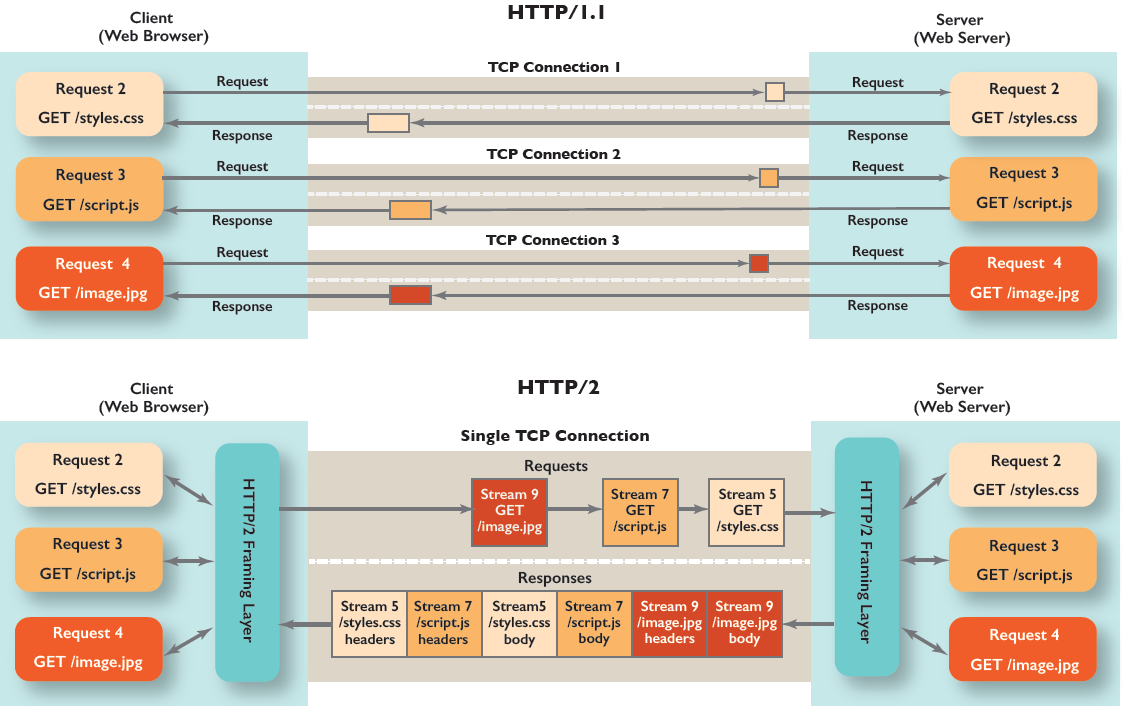
\includegraphics[width=\linewidth]{http.png}
  \caption{Visuele voorstelling van het verschil tussen het proces van een HTTP/1.1 en HTTP/2 verzoek, gemaakt door \cite{pollard_2018}}
  \label{fig:HttpComparison}
\end{figure*}

De bundlers die bekeken zullen worden in deze paper zijn als volgt:

\begin{itemize}
    \item Webpack
    \item ESBuild
    \item Vite
    \item Parcel
    \item Rollup
\end{itemize}

% Voor literatuurverwijzingen zijn er twee belangrijke commando's:
% \autocite{KEY} => (Auteur, jaartal) Gebruik dit als de naam van de auteur
%   geen onderdeel is van de zin.
% \textcite{KEY} => Auteur (jaartal)  Gebruik dit als de auteursnaam wel een
%   functie heeft in de zin (bv. ``Uit onderzoek door Doll & Hill (1954) bleek
%   ...'')


%---------- Methodologie ------------------------------------------------------
\section{Methodologie}
\label{sec:methodologie}

De transpilers en bundlers zullen beoordeeld worden gebaseerd op volgende criteria:

\begin{itemize}
  \item Snelheid
  \item Gebruiksvriendelijkheid
  \item Functionaliteit
  \item Huidige marktdominantie
\end{itemize}

Om de snelheid te beoordelen zullen voor elke transpiler en bundler benchmarks opgesteld worden aan de hand van met TypeScript opgestelde React applicaties van variërende groottes. De resultaten van deze benchmarks zullen geanalyseerd en vergeleken worden. Deze methodologie is geïnspireerd uit de methodes gebruikt in de analyse van \textcite{eaton_2021}. Vergeleken met de vooraf genoemde analyse, zullen hier meer nog pakketten vergeleken worden. Ook de reeds verkregen resultaten van die analyse zullen vergeleken kunnen worden met de resultaten van dit onderzoek.

Gebruiksvriendelijkheid zal beoordeeld worden aan de hand van een anonieme steekproef voor React developers, waar hun ervaringen met de transpilers en bundlers verzameld zullen worden.
De informatie die de onderzoeker tracht te achterhalen bevindt zich in tabel \ref{table:1}.
Ook overige externe bronnen die de gebruiksvriendelijkheid van deze pakketten bespreken kunnen gebruikt worden in de literatuurstudie om te helpen een duidelijkere conclusie te maken. Door de subjectieve aard van dit criterium is het alsnog ook mogelijk dat de eindconclusie van dit onderzoek er weinig of niet door beïnvloed zal worden. Dit zal worden bepaald door de onderzoeker aan de hand van de resultaten van de vragenlijst. De resultaten zullen echter hoe dan ook toegelicht worden.

\begin{table}[ht]
\begin{tabular}{|p{56mm}|l|}
\hline
\multicolumn{2}{|c|}{\textbf{Onafhankelijke variabelen}}         \\ \hline
\textbf{Variabele}                         & \textbf{Meetniveau} \\ \hline
Welke frameworks/libraries worden in de werkomgeving gebruikt& Nominaal\\ \hline
Gekende bundlers/transpilers               & Nominaal            \\ \hline
Uren ervaring per bundler/transpiler die in het laatste jaar gebruikt is& Ratio\\ \hline
Geobserveerde gebruiksvriendelijkheid per gebruikte bundler/transpiler& Ordinaal\\ \hline
Meest passende positieve kenmerk per gebruikte bundler/transpiler& Nominaal\\ \hline
Meest passende negatieve kenmerk per gebruikte bundler/transpiler& Nominaal\\ \hline
Eerste keuze bundler en transpiler in een nieuw project& Nominaal\\ \hline
Best-to-worst rangschikking van de gebruikte bundlers/transpiler& Ordinaal\\ \hline
\end{tabular}
\caption{Tabel van de informatie die achterhaalt tracht te worden door de vragenlijst.}
\label{table:1}
\end{table}

Functionaliteit wordt beoordeeld in het perspectief van React ontwikkeling. Missende of extra functionaliteit die een meerwaarde biedt aan ontwikkeling binnen React zal hier van het grootste belang zijn.

Marktdominantie zal gepeild worden aan de hand van data beschikbaar op NPM\footnote{Node Package Manager, ook gekend als NPM is de grootste repository voor JavaScript libraries}. Marktdominantie heeft onder andere een invloed op de ondersteuning van de onderhouders, de kwaliteit en kwantiteit van documentatie, en hoe waarschijnlijk het is dat een ontwikkelaar voorkennis heeft van de package.

Verder zal er ook aan de hand van praktische proeven bekeken worden welke transpilers en bundlers een eventuele goede samenwerking hebben met elkaar. Het is immers mogelijk dat één transpiler zich vestigt als de snellere, terwijl een tegenhanger veel betere samenwerking heeft met een bepaald bundler. Dit kan tot verandering leiden in de eindconclusie.

Om de beste combinaties tussen bundler en transpiler te identificeren binnen Codifly, zal er een individuele bevraging gebeuren om hun noden en prioriteiten vast te leggen.

Ten slotte zal een proof-of-concept opgesteld worden om de als best beschouwde combinatie in het spotlicht te zetten, en zo aan te tonen dat die combinatie aan te raden valt voor regelmatig gebruik binnen Codifly indien dit niet reeds het geval is.

%---------- Verwachte resultaten ----------------------------------------------
\section{Verwachte resultaten}
\label{sec:verwachte_resultaten}

\begin{figure*}[!htp]
  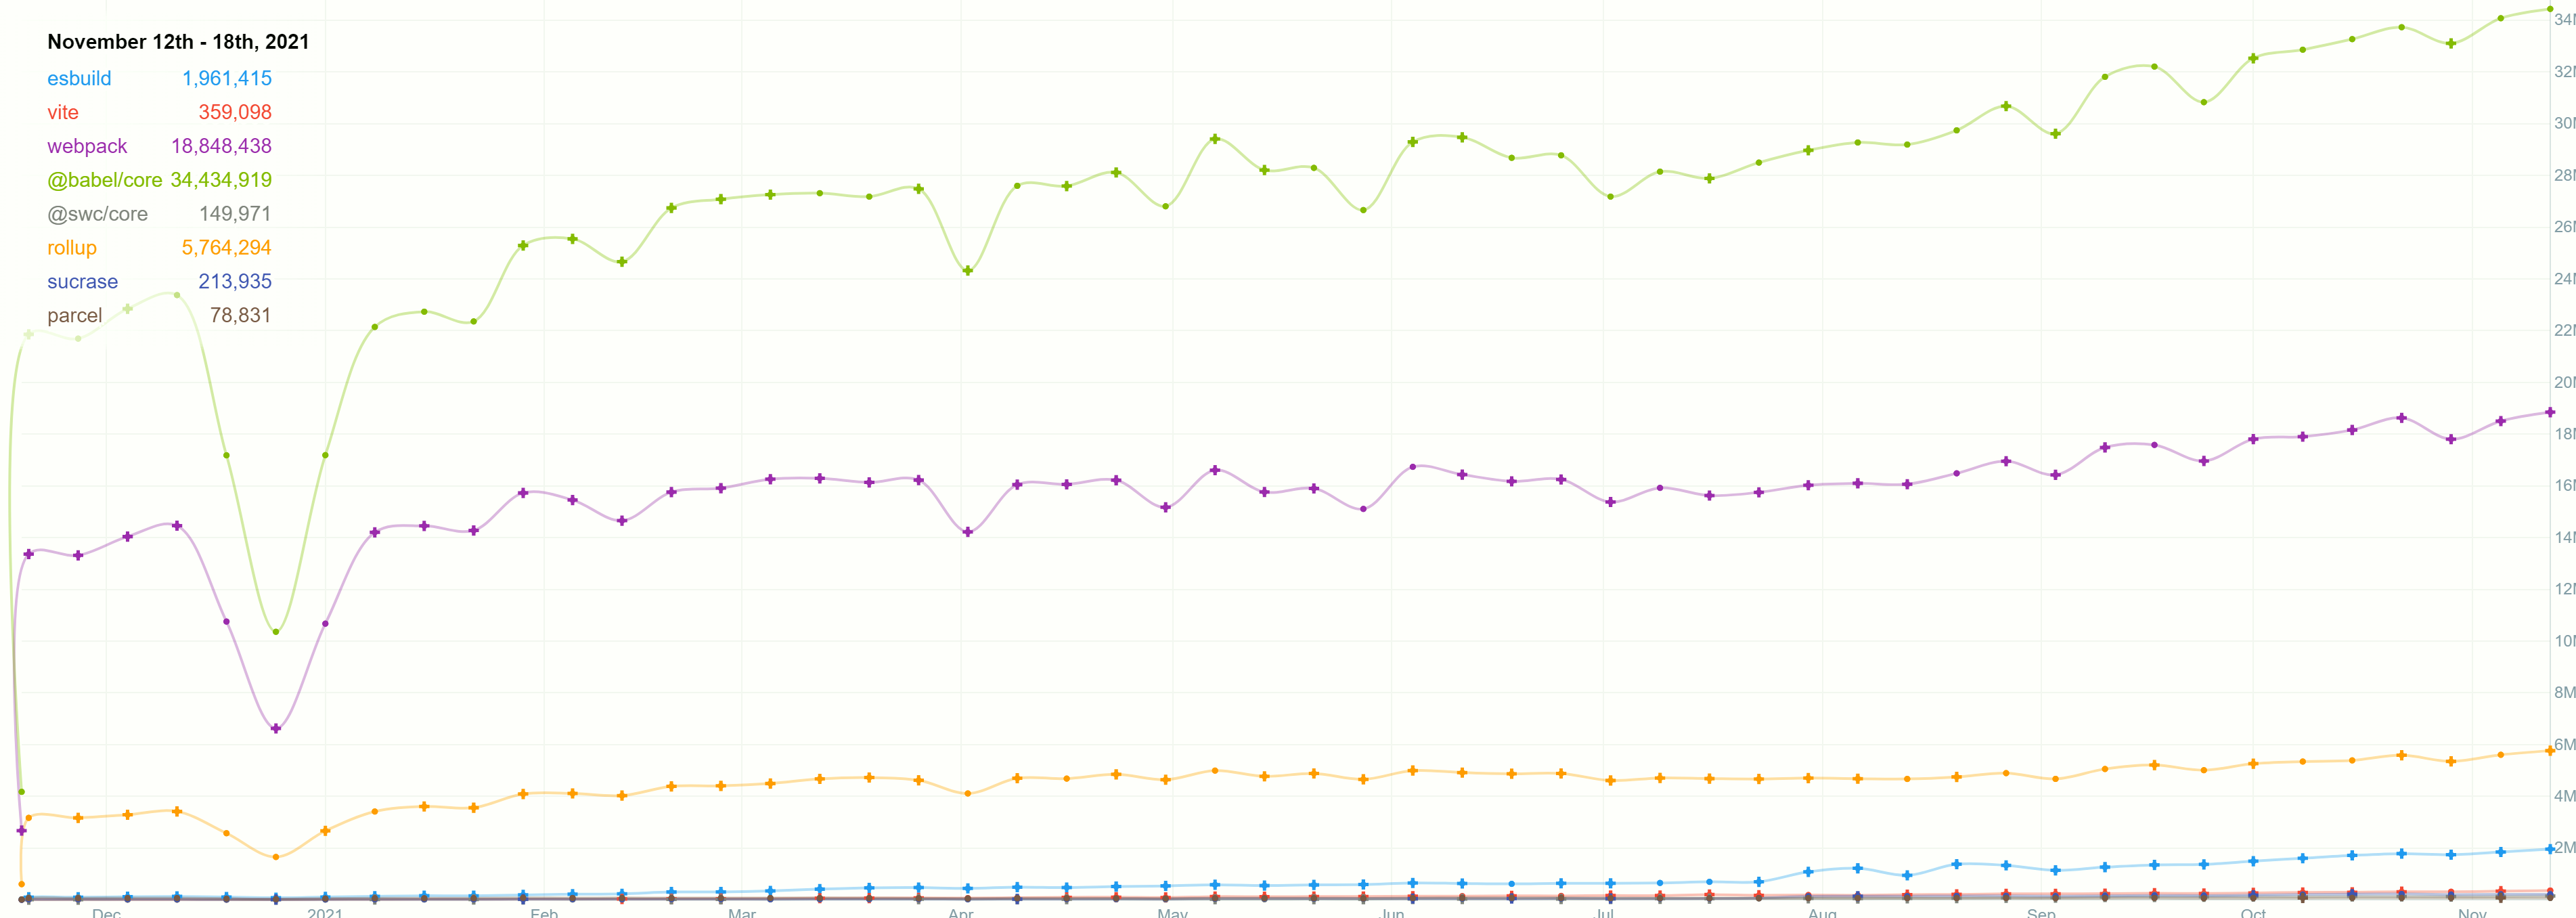
\includegraphics[width=\linewidth]{npmgraph.png}
  \caption{Lijndiagram van het aantal downloads van alle te onderzoeken bundlers en transpilers, behalve TSC. TSC is ingebouwd in TypeScript.}
  \label{fig:NpmDownloadsLineChart}
\end{figure*}

Populaire opties zoals bijvoorbeeld Babel en Webpack zijn niet altijd de snelste, maar hebben meer documentatie om mee te werken. Het is dan ook verwacht dat populairdere transpilers en bundlers eerder naar de gebruiksvriendelijke kant zullen leunen, terwijl de jongere en volop groeiende transpilers en bundlers sneller zullen zijn. Maar mogelijks met het nadeel van minder, of minder duidelijke documentatie. Uit figuur \ref{fig:NpmDownloadsLineChart} kunnen de populariteitstrends voor bijna alle transpilers en bundlers geïdentificeerd worden, wat hoogstwaarschijnlijk in de steekproef gereflecteerd zal worden.

%---------- Verwachte conclusies ----------------------------------------------
\section{Verwachte conclusies}
\label{sec:verwachte_conclusies}

Elke bundler en transpiler heeft een licht verschillende set van doelen die de maintainers willen bereiken. Er is dan echter ook waarschijnlijk geen één beste keuze die gemaakt kan worden op algemeen vlak. Binnen Codifly moet echter eerst achterhaald worden waar hun prioriteiten liggen bij de keuze van transpiler en bundler. Afhankelijk van de ondervindingen zal het antwoord nog veel kunnen variëren. 

De onderzoeker verwacht dat de rijpere projecten enige voorkeur zullen hebben, omwille van het feit dat die momenteel al in gebruik zijn, een goede basis hebben aan documentatie en een vollediger arsenaal hebben aan features.

Verder is er ook enige onzekerheid of dit onderzoek een werkelijk betere optie zal kunnen formuleren voor Codifly. Wanneer frameworks zoals Next.js in gebruik genomen worden is het ook niet altijd zo simpel om de bijgeleverde bundler en transpiler zomaar te vervangen. Voor projecten waar echter niet gebruik gemaakt wordt van een React framework zou dit niet het geval zijn.


%------------------------------------------------------------------------------
% Referentielijst
%------------------------------------------------------------------------------
% TODO: de gerefereerde werken moeten in BibTeX-bestand ``voorstel.bib''
% voorkomen. Gebruik JabRef om je bibliografie bij te houden en vergeet niet
% om compatibiliteit met Biber/BibLaTeX aan te zetten (File > Switch to
% BibLaTeX mode)

\phantomsection
\printbibliography[heading=bibintoc]

\end{document}
